\documentclass[tikz,border=0pt]{standalone}
\usepackage[T1]{fontenc}
\usepackage{newtxtext,newtxmath}
\usepackage{xcolor}
\definecolor{blue}{HTML}{326C9B}
\definecolor{gray}{HTML}{7F8993}
\definecolor{ink}{HTML}{203244}
\definecolor{grid}{HTML}{E5EAF0}
\definecolor{yellow}{HTML}{FFF19A}
\definecolor{orange}{HTML}{BD8547}
\definecolor{teal}{HTML}{488E85}
\usetikzlibrary{patterns}
\begin{document}
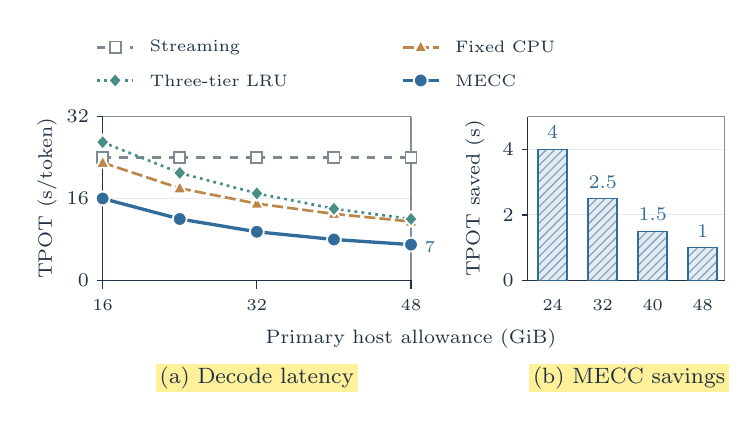
\begin{tikzpicture}[x=1bp,y=-1bp,every node/.style={inner sep=0pt,outer sep=0pt,text=ink,font=\fontsize{7.2}{8.2}\selectfont}]
\path[use as bounding box] (0,0) rectangle (252,132);
\draw[gray,line width=1.1bp,dashed] (25.000,7.000)--(38.000,7.000);
\filldraw[fill=white,draw=gray,line width=.65bp] (29.500,5.000) rectangle (33.500,9.000);
\node[anchor=west,text=ink,font=\fontsize{6.5}{7.5}\selectfont] at (44.000,7.000) {Streaming};
\draw[orange,line width=1.1bp,dash pattern=on 4bp off 1.5bp] (135.000,7.000)--(148.000,7.000);
\filldraw[fill=orange,draw=white,line width=.65bp] (141.500,4.400)--(139.100,8.800)--(143.900,8.800)--cycle;
\node[anchor=west,text=ink,font=\fontsize{6.5}{7.5}\selectfont] at (154.000,7.000) {Fixed CPU};
\draw[teal,line width=1.1bp,dash pattern=on 1bp off 1.5bp] (25.000,19.000)--(38.000,19.000);
\filldraw[fill=teal,draw=white,line width=.65bp] (31.500,16.300)--(29.100,19.000)--(31.500,21.700)--(33.900,19.000)--cycle;
\node[anchor=west,text=ink,font=\fontsize{6.5}{7.5}\selectfont] at (44.000,19.000) {Three-tier LRU};
\draw[blue,line width=1.1bp] (135.000,19.000)--(148.000,19.000);
\filldraw[fill=blue,draw=white,line width=.65bp] (141.500,19.000) circle[radius=2.5bp];
\node[anchor=west,text=ink,font=\fontsize{6.5}{7.5}\selectfont] at (154.000,19.000) {MECC};
\draw[grid,line width=0.35bp] (27.000,91.000)--(138.000,91.000);
\draw[ink,line width=0.45bp] (25.000,91.000)--(27.000,91.000);
\node[anchor=east,text=ink,font=\fontsize{6.7}{7.7}\selectfont] at (22.000,91.000) {0};
\draw[grid,line width=0.35bp] (27.000,61.500)--(138.000,61.500);
\draw[ink,line width=0.45bp] (25.000,61.500)--(27.000,61.500);
\node[anchor=east,text=ink,font=\fontsize{6.7}{7.7}\selectfont] at (22.000,61.500) {16};
\draw[grid,line width=0.35bp] (27.000,32.000)--(138.000,32.000);
\draw[ink,line width=0.45bp] (25.000,32.000)--(27.000,32.000);
\node[anchor=east,text=ink,font=\fontsize{6.7}{7.7}\selectfont] at (22.000,32.000) {32};
\draw[ink!55,line width=0.4bp] (27.000,32.000)--(138.000,32.000);
\draw[ink!55,line width=0.4bp] (138.000,32.000)--(138.000,91.000);
\draw[ink,line width=0.5bp] (27.000,32.000)--(27.000,91.000);
\draw[ink,line width=0.5bp] (27.000,91.000)--(138.000,91.000);
\draw[gray,line width=0.95bp,dashed] (27.000,46.750)--(54.750,46.750);
\draw[gray,line width=0.95bp,dashed] (54.750,46.750)--(82.500,46.750);
\draw[gray,line width=0.95bp,dashed] (82.500,46.750)--(110.250,46.750);
\draw[gray,line width=0.95bp,dashed] (110.250,46.750)--(138.000,46.750);
\filldraw[fill=white,draw=gray,line width=.65bp] (25.000,44.750) rectangle (29.000,48.750);
\filldraw[fill=white,draw=gray,line width=.65bp] (52.750,44.750) rectangle (56.750,48.750);
\filldraw[fill=white,draw=gray,line width=.65bp] (80.500,44.750) rectangle (84.500,48.750);
\filldraw[fill=white,draw=gray,line width=.65bp] (108.250,44.750) rectangle (112.250,48.750);
\filldraw[fill=white,draw=gray,line width=.65bp] (136.000,44.750) rectangle (140.000,48.750);
\draw[orange,line width=0.95bp,dash pattern=on 4bp off 1.5bp] (27.000,48.594)--(54.750,57.812);
\draw[orange,line width=0.95bp,dash pattern=on 4bp off 1.5bp] (54.750,57.812)--(82.500,63.344);
\draw[orange,line width=0.95bp,dash pattern=on 4bp off 1.5bp] (82.500,63.344)--(110.250,67.031);
\draw[orange,line width=0.95bp,dash pattern=on 4bp off 1.5bp] (110.250,67.031)--(138.000,69.797);
\filldraw[fill=orange,draw=white,line width=.65bp] (27.000,45.994)--(24.600,50.394)--(29.400,50.394)--cycle;
\filldraw[fill=orange,draw=white,line width=.65bp] (54.750,55.212)--(52.350,59.612)--(57.150,59.612)--cycle;
\filldraw[fill=orange,draw=white,line width=.65bp] (82.500,60.744)--(80.100,65.144)--(84.900,65.144)--cycle;
\filldraw[fill=orange,draw=white,line width=.65bp] (110.250,64.431)--(107.850,68.831)--(112.650,68.831)--cycle;
\filldraw[fill=orange,draw=white,line width=.65bp] (138.000,67.197)--(135.600,71.597)--(140.400,71.597)--cycle;
\draw[teal,line width=0.95bp,dash pattern=on 1bp off 1.5bp] (27.000,41.219)--(54.750,52.281);
\draw[teal,line width=0.95bp,dash pattern=on 1bp off 1.5bp] (54.750,52.281)--(82.500,59.656);
\draw[teal,line width=0.95bp,dash pattern=on 1bp off 1.5bp] (82.500,59.656)--(110.250,65.188);
\draw[teal,line width=0.95bp,dash pattern=on 1bp off 1.5bp] (110.250,65.188)--(138.000,68.875);
\filldraw[fill=teal,draw=white,line width=.65bp] (27.000,38.519)--(24.600,41.219)--(27.000,43.919)--(29.400,41.219)--cycle;
\filldraw[fill=teal,draw=white,line width=.65bp] (54.750,49.581)--(52.350,52.281)--(54.750,54.981)--(57.150,52.281)--cycle;
\filldraw[fill=teal,draw=white,line width=.65bp] (82.500,56.956)--(80.100,59.656)--(82.500,62.356)--(84.900,59.656)--cycle;
\filldraw[fill=teal,draw=white,line width=.65bp] (110.250,62.487)--(107.850,65.188)--(110.250,67.888)--(112.650,65.188)--cycle;
\filldraw[fill=teal,draw=white,line width=.65bp] (138.000,66.175)--(135.600,68.875)--(138.000,71.575)--(140.400,68.875)--cycle;
\draw[blue,line width=1.2bp] (27.000,61.500)--(54.750,68.875);
\draw[blue,line width=1.2bp] (54.750,68.875)--(82.500,73.484);
\draw[blue,line width=1.2bp] (82.500,73.484)--(110.250,76.250);
\draw[blue,line width=1.2bp] (110.250,76.250)--(138.000,78.094);
\filldraw[fill=blue,draw=white,line width=.65bp] (27.000,61.500) circle[radius=2.5bp];
\filldraw[fill=blue,draw=white,line width=.65bp] (54.750,68.875) circle[radius=2.5bp];
\filldraw[fill=blue,draw=white,line width=.65bp] (82.500,73.484) circle[radius=2.5bp];
\filldraw[fill=blue,draw=white,line width=.65bp] (110.250,76.250) circle[radius=2.5bp];
\filldraw[fill=blue,draw=white,line width=.65bp] (138.000,78.094) circle[radius=2.5bp];
\draw[ink,line width=0.45bp] (27.000,91.000)--(27.000,94.000);
\node[anchor=center,text=ink,font=\fontsize{6.5}{7.5}\selectfont] at (27.000,100.000) {16};
\draw[ink,line width=0.45bp] (82.500,91.000)--(82.500,94.000);
\node[anchor=center,text=ink,font=\fontsize{6.5}{7.5}\selectfont] at (82.500,100.000) {32};
\draw[ink,line width=0.45bp] (138.000,91.000)--(138.000,94.000);
\node[anchor=center,text=ink,font=\fontsize{6.5}{7.5}\selectfont] at (138.000,100.000) {48};
\node[anchor=center,text=ink,font=\fontsize{7}{8}\selectfont,rotate=90] at (7.000,61.500) {TPOT (s/token)};
\node[anchor=west,text=blue,font=\fontsize{6.5}{7.5}\selectfont] at (143.000,79.094) {7};
\draw[grid,line width=0.35bp] (180.000,91.000)--(251.000,91.000);
\draw[ink,line width=0.45bp] (178.000,91.000)--(180.000,91.000);
\node[anchor=east,text=ink,font=\fontsize{6.7}{7.7}\selectfont] at (175.000,91.000) {0};
\draw[grid,line width=0.35bp] (180.000,67.400)--(251.000,67.400);
\draw[ink,line width=0.45bp] (178.000,67.400)--(180.000,67.400);
\node[anchor=east,text=ink,font=\fontsize{6.7}{7.7}\selectfont] at (175.000,67.400) {2};
\draw[grid,line width=0.35bp] (180.000,43.800)--(251.000,43.800);
\draw[ink,line width=0.45bp] (178.000,43.800)--(180.000,43.800);
\node[anchor=east,text=ink,font=\fontsize{6.7}{7.7}\selectfont] at (175.000,43.800) {4};
\draw[ink!55,line width=0.4bp] (180.000,32.000)--(251.000,32.000);
\draw[ink!55,line width=0.4bp] (251.000,32.000)--(251.000,91.000);
\draw[ink,line width=0.5bp] (180.000,32.000)--(180.000,91.000);
\draw[ink,line width=0.5bp] (180.000,91.000)--(251.000,91.000);
\fill[blue!13] (183.800,43.800) rectangle (194.200,91);
\fill[pattern=north east lines,pattern color=blue!65] (183.800,43.800) rectangle (194.200,91);
\draw[blue,line width=.55bp] (183.800,43.800) rectangle (194.200,91);
\node[anchor=center,text=blue,font=\fontsize{6.8}{7.8}\selectfont] at (189.000,37.800) {4};
\node[anchor=center,text=ink,font=\fontsize{6.5}{7.5}\selectfont] at (189.000,100.000) {24};
\fill[blue!13] (201.800,61.500) rectangle (212.200,91);
\fill[pattern=north east lines,pattern color=blue!65] (201.800,61.500) rectangle (212.200,91);
\draw[blue,line width=.55bp] (201.800,61.500) rectangle (212.200,91);
\node[anchor=center,text=blue,font=\fontsize{6.8}{7.8}\selectfont] at (207.000,55.500) {2.5};
\node[anchor=center,text=ink,font=\fontsize{6.5}{7.5}\selectfont] at (207.000,100.000) {32};
\fill[blue!13] (219.800,73.300) rectangle (230.200,91);
\fill[pattern=north east lines,pattern color=blue!65] (219.800,73.300) rectangle (230.200,91);
\draw[blue,line width=.55bp] (219.800,73.300) rectangle (230.200,91);
\node[anchor=center,text=blue,font=\fontsize{6.8}{7.8}\selectfont] at (225.000,67.300) {1.5};
\node[anchor=center,text=ink,font=\fontsize{6.5}{7.5}\selectfont] at (225.000,100.000) {40};
\fill[blue!13] (237.800,79.200) rectangle (248.200,91);
\fill[pattern=north east lines,pattern color=blue!65] (237.800,79.200) rectangle (248.200,91);
\draw[blue,line width=.55bp] (237.800,79.200) rectangle (248.200,91);
\node[anchor=center,text=blue,font=\fontsize{6.8}{7.8}\selectfont] at (243.000,73.200) {1};
\node[anchor=center,text=ink,font=\fontsize{6.5}{7.5}\selectfont] at (243.000,100.000) {48};
\node[anchor=center,text=ink,font=\fontsize{6.9}{7.9}\selectfont,rotate=90] at (161.000,61.500) {TPOT saved (s)};
\node[anchor=center,text=ink,font=\fontsize{6.9}{7.9}\selectfont] at (138.000,112.000) {Primary host allowance (GiB)};
\node[anchor=center,text=ink,font=\fontsize{7.8}{8.8}\selectfont,fill=yellow,inner xsep=1.4bp,inner ysep=1.0bp] at (82.500,126.000) {(a) Decode latency};
\node[anchor=center,text=ink,font=\fontsize{7.8}{8.8}\selectfont,fill=yellow,inner xsep=1.4bp,inner ysep=1.0bp] at (216.500,126.000) {(b) MECC savings};
\end{tikzpicture}
\end{document}
